% Gemini theme
% https://github.com/anishathalye/gemini
%
% We try to keep this Overleaf template in sync with the canonical source on
% GitHub, but it's recommended that you obtain the template directly from
% GitHub to ensure that you are using the latest version.

\documentclass[final, 20pt]{beamer}

% ====================
% Packages
% ====================

\usepackage[T1]{fontenc}
\usepackage{lmodern}
% \usepackage[size=custom,width=120,height=72,scale=1.0]{beamerposter}
\usepackage[size=a1,scale=1.3]{beamerposter}
\usetheme{gemini}
\usecolortheme{gemini}
\usepackage{graphicx}
\graphicspath{ {./images/} }
\usepackage{booktabs}
\usepackage{tikz}
\usepackage{pgfplots}
\usepackage{subfig}
\usepackage[export]{adjustbox}
\usepackage{wrapfig}
\usepackage{lipsum}
% ====================
% Lengths
% ====================

% If you have N columns, choose \sepwidth and \colwidth such that
% (N+1)*\sepwidth + N*\colwidth = \paperwidth
\newlength{\sepwidth}
\newlength{\colwidth}
\setlength{\sepwidth}{0.025\paperwidth}
\setlength{\colwidth}{0.3\paperwidth}

\newcommand{\separatorcolumn}{\begin{column}{\sepwidth}\end{column}}

% ====================
% Title
% ====================

\title{Construction/Operation of Two Hexacopters for Autonomous Landing}

\author{Joshua Springer}

\institute[shortinst]{Reykjavík University}

% ====================
% Body
% ====================

\begin{document}

\begin{frame}[t]
\begin{columns}[t]
\separatorcolumn

\begin{column}{\colwidth}

  \begin{block}{Overview}
    Two Tarot 680 Hexacopters enable real world testing of autonomous navigation techniques developed in simulation.
    This project tests an autonomous landing algorithm based on computer vision and fiducial markers.\cite{AL_thesis}
    A landing pad is marked with fiducial markers which are recognized by the drone's onboard camera.
    The gimbal automatically aims the camera at the landing pad to track it during descent.
    The landing software then directs the drone to descend towards the landing pad.
  \end{block}

  \begin{alertblock}{Components}

    \heading{Standard Drone Components}
    All drone electronics (e.g. motors, speed controllers, propellers, power electronics, RC Receiver, telemetry radio) are mounted on the Tarot 680 Pro hexacopter body.

    \heading{Computational Components}
    \begin{itemize}
      \item \textbf{Raspberry Pi 3 B+:} runs the ArduPilot flight software and ROS.
      \item \textbf{Navio2 Hat:} provides IMU data and control signal interfaces.
      \item \textbf{Companion board:} image processing, fiducial marker systems, coordinate system transforms. One drone uses a Google Coral Dev board and the other uses an NVIDIA Jetson Nano.
    \end{itemize}

    \begin{figure}
      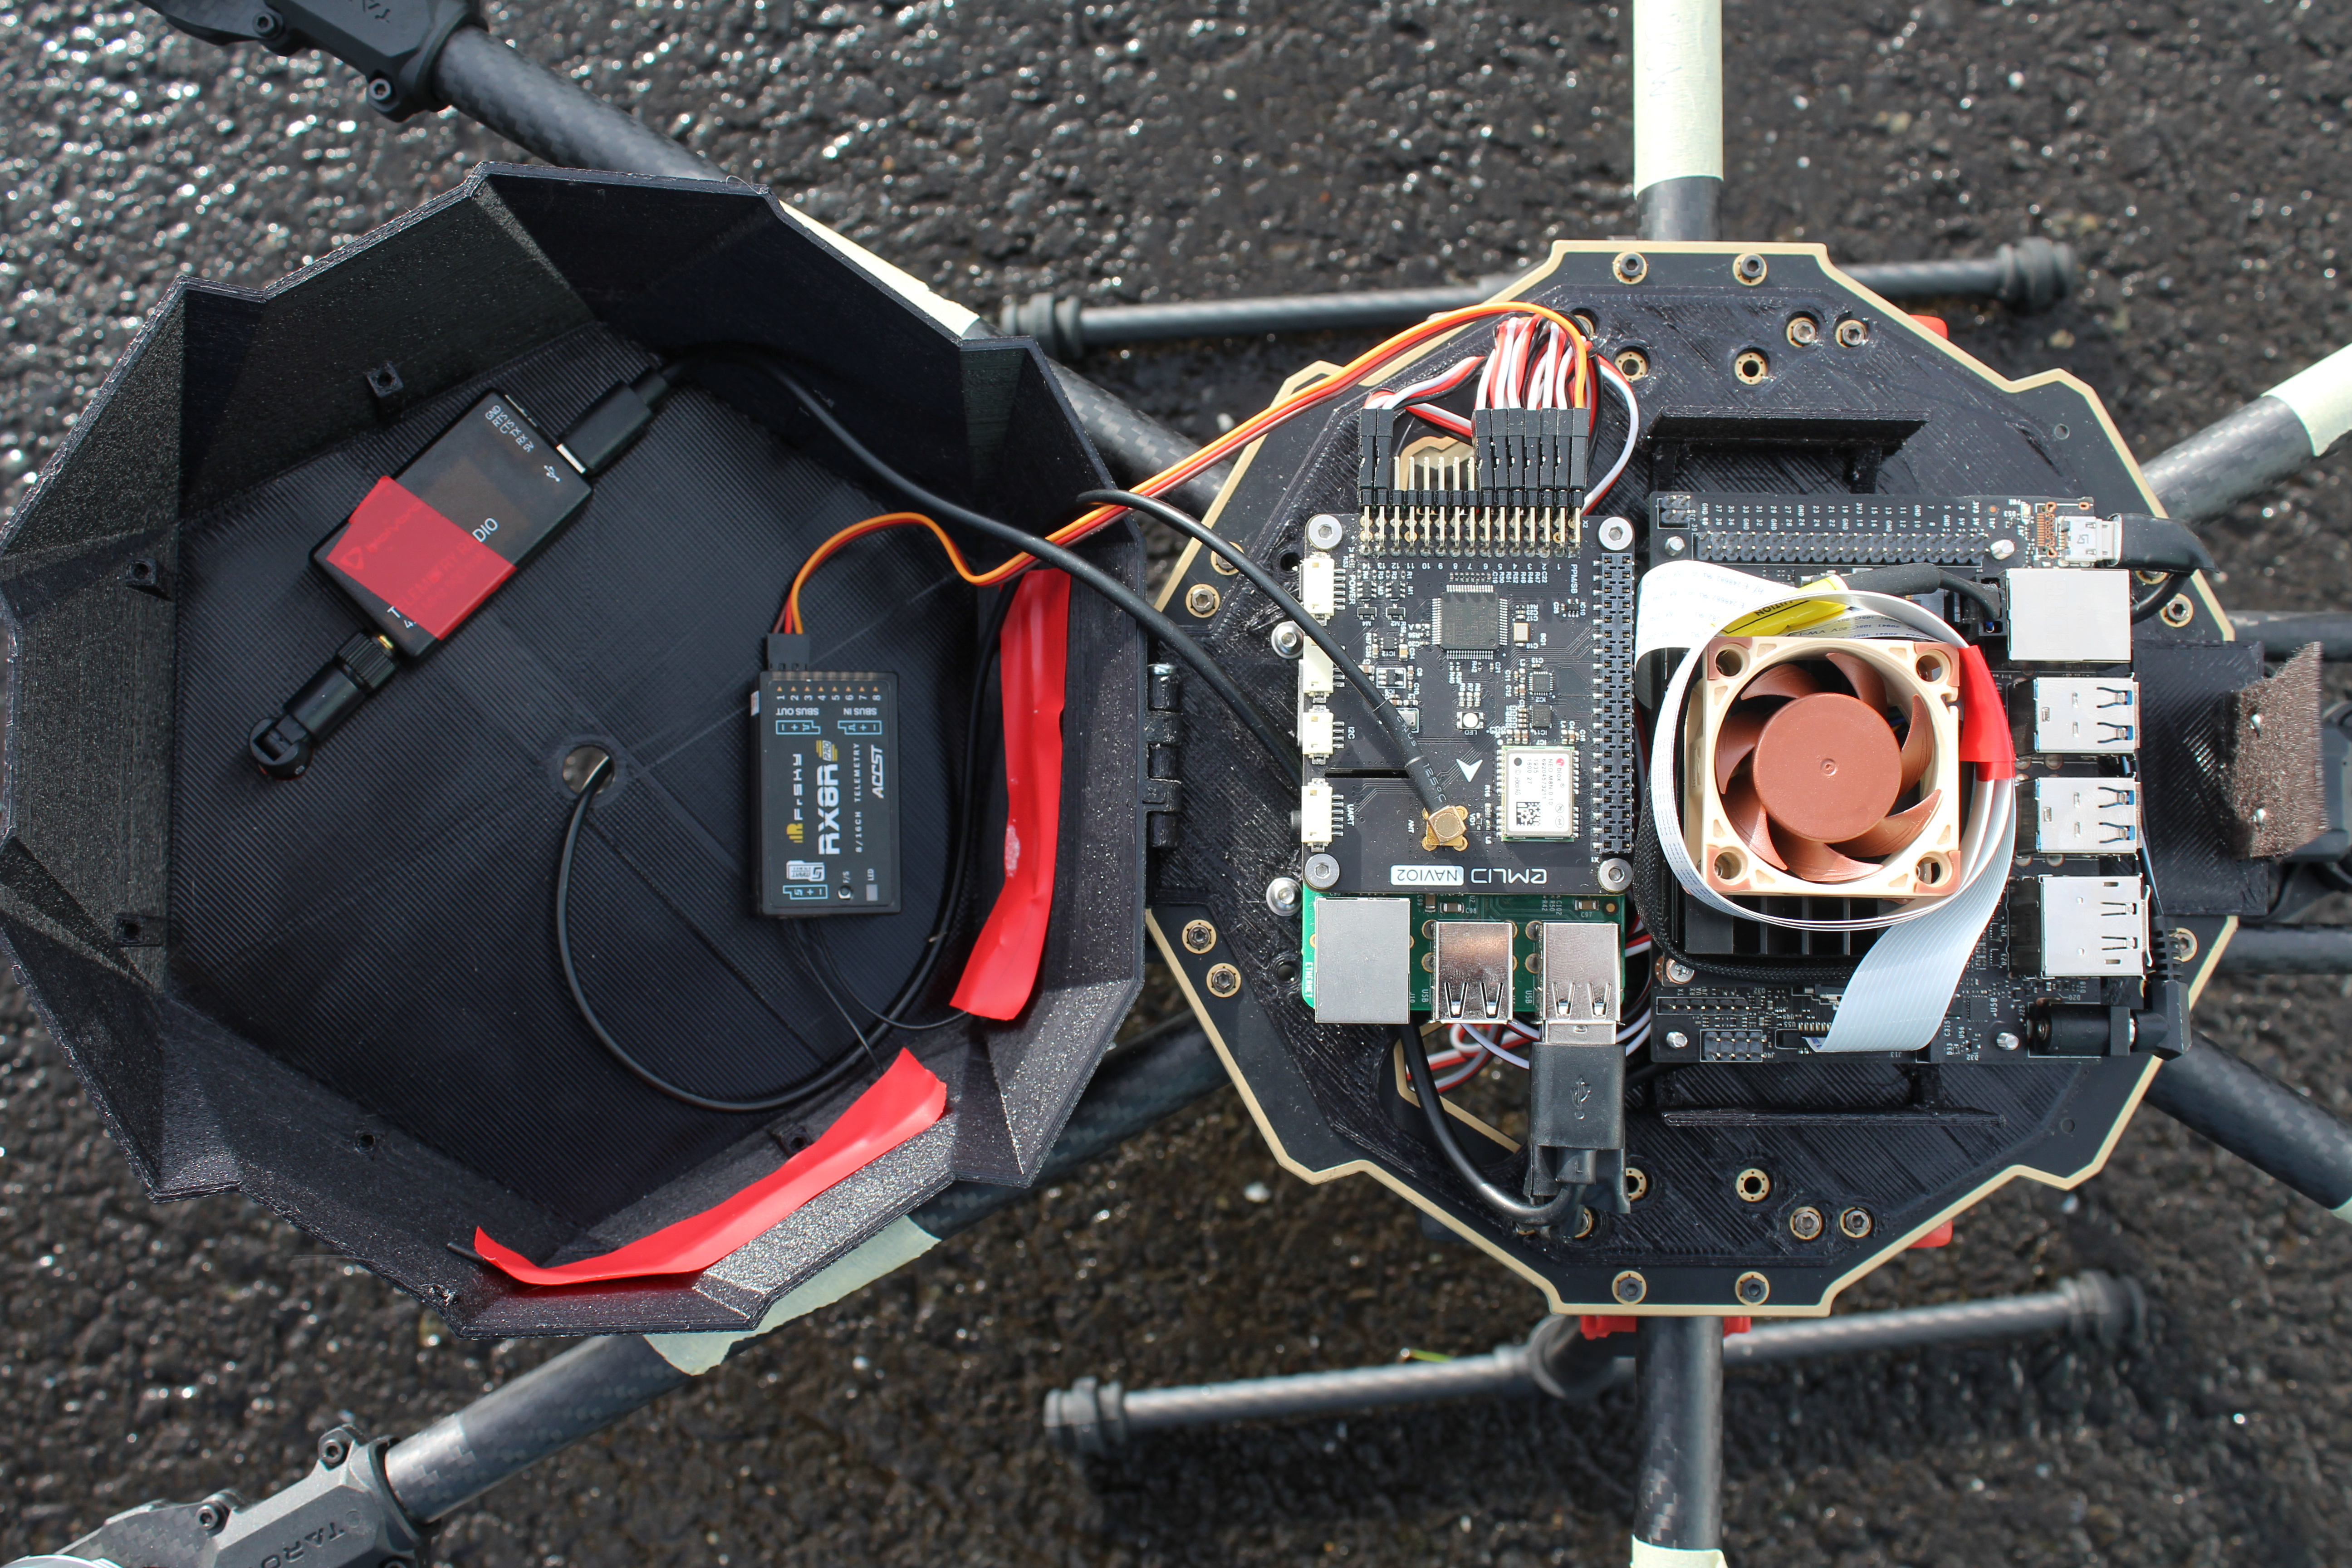
\includegraphics[width=0.45\linewidth]{jetson_electronics}
      \includegraphics[width=0.45\linewidth]{jetson_drone.jpg}
    \end{figure}

    \heading{Custom 3D-Printed Components}

    \begin{figure}
      \centering
      \subfloat[Protective canopy.]{\label{figur:1}\includegraphics[width=0.3\textwidth]{canopy.png}}
      \hspace{1cm}
      \subfloat[Component mounting plate.]{\label{figur:1}\includegraphics[width=0.3\textwidth]{component_mounting_plate.png}}
      \\
      \subfloat[Google Coral camera case.]{\label{figur:1}\includegraphics[width=0.3\textwidth]{coral_case.png}}
      \hspace{1cm}
      \subfloat[Jetson Nano camera case.]{\label{figur:1}\includegraphics[width=0.3\textwidth]{nano_case.png}}
    \end{figure}
  \end{alertblock}

\end{column}

\separatorcolumn

\begin{column}{\colwidth}

  \begin{block}{Power and Data Flow}
        The drones have two power systems to isolate the computational electronics from voltage spikes/drops caused by the motors and gimbal.
        \begin{figure}
          \includegraphics[width=0.6\textwidth]{hardware.png}
%          \caption{Power flow and control signals.}
        \end{figure}

        \vspace{-1.5cm}
        \heading{Data Flow}
        \begin{itemize}
          \item \textbf{Camera module:} provides a high-quality video image.
          \item \textbf{\texttt{gscam}:} pre-processes the image (lowering resolution, flipping).
          \item \textbf{\texttt{landing\_controller}:} generates a target position for the drone.
          \item \textbf{\texttt{gimbal\_controller}:} tracks the landing pad by aiming the camera.
          \item \textbf{MAVROS:} translates ROS messages to ArduPilot messages.
          \item \textbf{ArduPilot:} controls the drone based on MAVROS commands.
        \end{itemize}

        \begin{figure}
            \includegraphics[width=0.9\textwidth]{data_flow.png}
        \end{figure}
  \end{block}

  \begin{block}{Landing Pad}

    \begin{wrapfigure}{r}{8cm}
      \fbox{\includegraphics[angle=180, width=8cm]{landing_pad.png}}
%      \caption*{Initial landing pad design.}
    \end{wrapfigure}

    Fiducial markers (top: April Tag\cite{apriltag_paper}, bottom: WhyCon\cite{whycon_paper}) allow the drone to determine its position relative to the landing pad using only a normal RGB camera.

    \begin{itemize}
      \item \textbf{April Tag:} provides accurate pose estimation at close range, when the WhyCon marker is too big for the camera to fully see. Eventually it was abandoned for consuming excessive CPU time.
      \item \textbf{WhyCon:} provide easier/faster recognition at long range. The center of the WhyCon marker is the target landing site.
    \end{itemize}

%    The larger WhyCon marker is easier for the system to recognize at long range, while the April Tag marker provides more accurate pose estimates at close range.
%    The April Tag marker is positioned in front of the WhyCon marker in order to keep it in the field of view of the camera at close range.
%    The drone touches down in the center of the WhyCon marker.
%    Eventually the April Tag marker was abandoned for consuming excessive processing power.

  \end{block}

\end{column}

\separatorcolumn

\begin{column}{\colwidth}

  \begin{alertblock}{A block containing some math}

    Nullam non est elit. In eu ornare justo. Maecenas porttitor sodales lacus,
    ut cursus augue sodales ac.

    $$
    \int_{-\infty}^{\infty} e^{-x^2}\,dx = \sqrt{\pi}
    $$

    Interdum et malesuada fames $\{1, 4, 9, \ldots\}$ ac ante ipsum primis in
    faucibus. Cras eleifend dolor eu nulla suscipit suscipit. Sed lobortis non
    felis id vulputate.

    \heading{A heading inside a block}

    Praesent consectetur mi $x^2 + y^2$ metus, nec vestibulum justo viverra
    nec. Proin eget nulla pretium, egestas magna aliquam, mollis neque. Vivamus
    dictum $\mathbf{u}^\intercal\mathbf{v}$ sagittis odio, vel porta erat
    congue sed. Maecenas ut dolor quis arcu auctor porttitor.

    \heading{Another heading inside a block}

    Sed augue erat, scelerisque a purus ultricies, placerat porttitor neque.
    Donec $P(y \mid x)$ fermentum consectetur $\nabla_x P(y \mid x)$ sapien
    sagittis egestas. Duis eget leo euismod nunc viverra imperdiet nec id
    justo.

  \end{alertblock}

  \begin{block}{Nullam vel erat at velit convallis laoreet}

    Class aptent taciti sociosqu ad litora torquent per conubia nostra, per
    inceptos himenaeos. Phasellus libero enim, gravida sed erat sit amet,
    scelerisque congue diam. Fusce dapibus dui ut augue pulvinar iaculis.

    \begin{table}
      \centering
      \begin{tabular}{l r r c}
        \toprule
        \textbf{First column} & \textbf{Second column} & \textbf{Third column} & \textbf{Fourth} \\
        \midrule
        Foo & 13.37 & 384,394 & \alpha \\
        Bar & 2.17 & 1,392 & \beta \\
        Baz & 3.14 & 83,742 & \delta \\
        Qux & 7.59 & 974 & \gamma \\
        \bottomrule
      \end{tabular}
      \caption{A table caption.}
    \end{table}

  \end{block}

  \begin{block}{References}

%    \nocite{*}
    \bibliographystyle{ieeetr}
    \footnotesize{\bibliography{poster}}

  \end{block}

\end{column}

\separatorcolumn
\end{columns}
\end{frame}

\end{document}
